 
\documentclass{beamer}            
\usepackage{beamerthemedefault, multimedia}            
\useoutertheme{smoothbars}            
\useinnertheme[shadow=true]{rounded}            
\setbeamercovered{transparent}            
\setbeamertemplate{navigation symbols}{}            
\setbeamertemplate{footline}[frame number]            
\usepackage{graphicx}            
\usepackage{morefloats}            
\usepackage{amsmath}            
\usepackage{amssymb}            
\usepackage{rotating}            
% mcode options for matlab code insertion bw (for printing), numbered (line numbers), framed (frame around code blocks), useliterate (convert Matlab expressions to Latex ones), autolinebreaks (automatic code wraping, use it with caution            
\usepackage[literate]{mcode}            
\graphicspath{{figures/}{tex/}{../figures/}{../../}{../}}             
\title{timbralSimilaritySolPerceptualProjectionSlides}            
\author{ Mathieu Lagrange }            
 
\begin{document}            
 
\maketitle            
 
% Please use this file to document your experiment            
% You can compile the report by setting the option 'report' as detailed in your expLanes configuration file.            
 
The first table compares the plain and joint scattering without any reprojection.           
\begin{enumerate}           
\item median: use median renormalization for scattering features           
\item compress: use log compression for scattering features           
\item standardize: standardize features at the end           
\end{enumerate}           
Use of all post processing give best performance. The second table show the results of using some projection. separateJudgment results can be seen as upper bound results.           
 
\begin{enumerate}           
\item averageJudgment: use cluster ensemble techniques http://strehl.com/soft.html to obtain one clustering. thus only one projection is computed           
\item separateJudgment: can be seen as an oracle method where each projection is evaluated using the clustering it has considered and average performance           
\end{enumerate}           
 
 
 
 
 
\begin{frame}\frametitle{Factors flow graph}          
 
 
\begin{center}         
 
 
\begin{figure}        
 
 
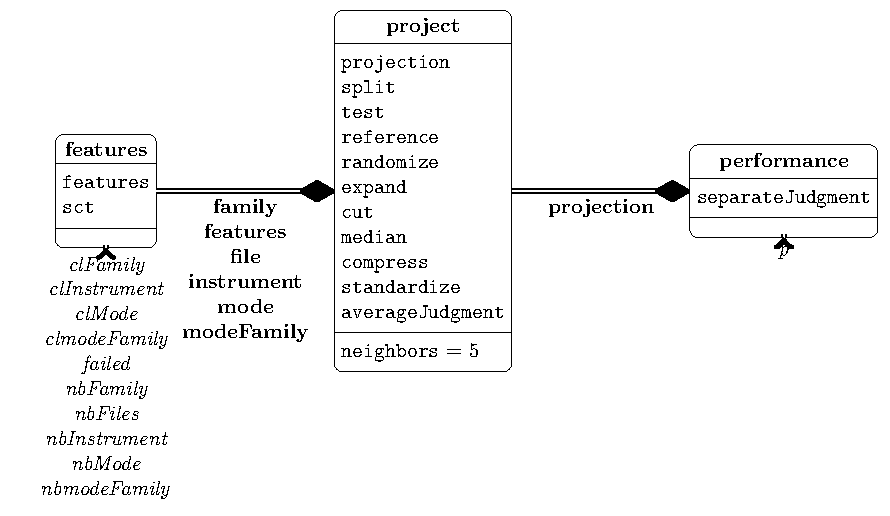
\includegraphics[width=\textwidth,height=0.8\textheight,keepaspectratio]{../figures/factors.pdf}       
 
 
\label{factorFlowGraph}      
 
 
\end{figure}     
 
 
\end{center}    
 
 
\end{frame}   
 
\begin{frame}\frametitle{features: tfscat, sct: 25, projection: none, split: none, reference: judgments, randomize: 0}  
 
\begin{table}  
\begin{center}  
\  
\setlength{\tabcolsep}{.16667em}  
\begin{tabular}{lllccccc}  
median & compress & standardize & p (\%) &  &  &  & p (\%) \\  
\hline  
0 & 0 & 0 & 69.25 $\pm$9.67 &  &  &  & 74.80 $\pm$8.67 \\  
0 & 0 & 1 & 76.65 $\pm$8.09 &  &  &  & 85.61 $\pm$5.56 \\  
0 & 1 & 0 & 81.92 $\pm$7.03 &  &  &  & \textbf{89.49 $\pm$4.30} \\  
0 & 1 & 1 & 81.49 $\pm$7.24 &  &  &  & \textbf{89.95 $\pm$4.08} \\  
1 & 0 & 0 & 76.99 $\pm$8.14 &  &  &  & 86.43 $\pm$5.36 \\  
1 & 0 & 1 & 76.65 $\pm$8.09 &  &  &  & 85.61 $\pm$5.56 \\  
1 & 1 & 0 & \textbf{85.70 $\pm$6.30} &  &  &  & \textbf{91.08 $\pm$3.83} \\  
1 & 1 & 1 & \textbf{\textcolor{red}{86.39 $\pm$6.13}} &  &  &  & \textbf{\textcolor{red}{91.12 $\pm$3.80}} \\  
\end{tabular}  
\end{center}  
\label{fetfSc25PrnoSpnoRejuRa0}  
\end{table}  
 
\end{frame}   
\begin{frame}\frametitle{features: tfscat, sct: 25, split: none, reference: judgments, randomize: 0, median: 1, compress: 1, standardize: 1} 
  
\begin{table} 
\begin{center} 
\ 
 \setlength{\tabcolsep}{.16667em} 
\begin{tabular}{lllccccc} 
pro & avejud & sepjud & p (\%) &  &  &  & p (\%) \\ 
\hline 
none & 1 & 0 & 86.39 $\pm$6.13 &  &  &  & 91.12 $\pm$3.80 \\ 
lmnn & 0 & 0 & 91.59 $\pm$4.66 &  &  &  & \textbf{96.20 $\pm$2.27} \\ 
lmnn & 0 & 1 & \textbf{\textcolor{red}{95.22 $\pm$3.23}} &  &  &  & \textbf{\textcolor{red}{96.89 $\pm$2.08}} \\ 
lmnn & 1 & 0 & 93.19 $\pm$3.84 &  &  &  & 95.60 $\pm$2.32 \\ 
lda & 1 & 0 & 82.40 $\pm$7.64 &  &  &  & 81.31 $\pm$8.51 \\ 
lda & 1 & 1 & 82.40 $\pm$7.64 &  &  &  & 81.31 $\pm$8.51 \\ 
\end{tabular} 
\end{center} 
\label{fetfSc25SpnoRejuRa0Me1Co1St1} 
\end{table} 
 
\end{frame}  
  
 
  
  
\begin{frame}\frametitle{Factors flow graph} 
  
  
\begin{center} 
  
  
\begin{figure} 
  
  
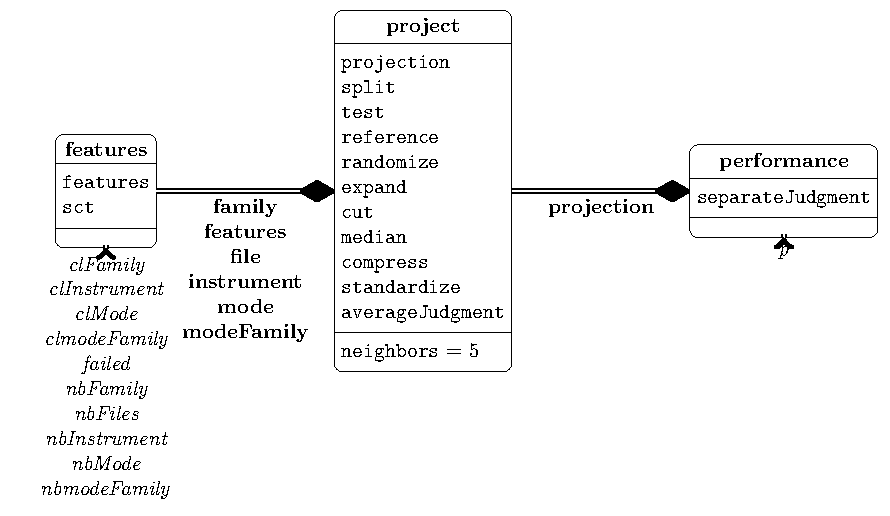
\includegraphics[width=\textwidth,height=0.8\textheight,keepaspectratio]{../figures/factors.pdf} 
  
  
\label{factorFlowGraph} 
  
  
\end{figure} 
  
  
\end{center} 
  
  
\end{frame} 
  
\begin{frame}\frametitle{sct: 25, projection: lmnn, split: none, reference: judgments, randomize: 0, expand: 0, cut: 1, median: 1, compress: 1, standardize: 1, averageJudgment: 0} 
  
\begin{table} 
\begin{center} 
\ 
 \setlength{\tabcolsep}{.16667em} 
\begin{tabular}{llc} 
fea & sepjud & p (\%) \\ 
\hline 
mfcc & 0 & 86.3 \\ 
mfcc & 1 & 86.2 \\ 
mfcc & 2 & 85.1 \\ 
scat & 0 & 91.6 \\ 
scat & 1 & 95.2 \\ 
scat & 2 & 86.4 \\ 
tfscat & 0 & \textbf{96.2} \\ 
tfscat & 1 & \textbf{\textcolor{red}{96.9}} \\ 
tfscat & 2 & 91.1 \\ 
\end{tabular} 
\end{center} 
\label{sc25PrlmSpnoRejuRa0Ex0Cu1Me1Co1St1Avju0} 
\end{table} 
 
\end{frame}  
 % expLanesInsertionFlag DO NOT CLEAR (but move it where you want the generated temporary LaTEX code to be inserted) 
 
 
\bibliographystyle{abbrvnat}            
\bibliography{bib}            
 
\end{document}            
